%% JAIHC version of the EngageNet engagement paper (Journal of Ambient Intelligence and Humanized Computing).
%% Journal rules (submission guidelines, checked 2026-10-01): \documentclass[iicol,sn-basic]{sn-jnl}, two columns,
%% author-year references, at most 12 pages INCLUDING references at submission (14 after revision), no
%% space-saving tricks, figure lettering similar in size to the running text, abstract 150-250 words, 4-6 keywords,
%% "Statements and Declarations", LLM use documented in the Methods.
%% Condensed from research/paper_springer/paper.tex (MTAP long version); every number traces to results/fullclip/
%% and results/paper_springer/ (scripts/paper/*.py); see docs/plan.md Sec. 18.16-18.17.
%% Before submission: replace each \input{figures/...} by the compiled figure PDF and paste the .bbl into this file.

\documentclass[pdflatex,iicol,sn-basic]{sn-jnl}

\usepackage{graphicx}
\graphicspath{{figures/}}
\usepackage{amsmath,amssymb,amsfonts}
\usepackage{xcolor}
\usepackage{booktabs}
\usepackage{tikz}
\usetikzlibrary{positioning,calc,decorations.pathreplacing}
\usepackage{pgfplots}
\pgfplotsset{compat=1.17}
% Shared figure colours (validated for colour-vision deficiency; see dataviz palette).
\definecolor{ours}{HTML}{2A78D6}      % our single models
\definecolor{fused}{HTML}{EB6834}     % our late fusion
\definecolor{published}{HTML}{8F8E88} % published EngageNet baselines
\definecolor{inkmuted}{HTML}{52514E}
\definecolor{boxfill}{HTML}{F3F2EF}
\definecolor{seqlo}{HTML}{FFFFFF}
\definecolor{seqhi}{HTML}{104281}


% Model name used throughout. Change it here only.
\newcommand{\ournet}{AVB-Engage}

\raggedbottom

\begin{document}

\title[Audio-visual and facial-behavior fusion for ordinal engagement recognition]{Audio-Visual Cross-Attention and Facial-Behavior Fusion for Ordinal Student Engagement Recognition in Online Learning}

% Author names withheld in this draft. The title page needs names, affiliations, the corresponding
% author's e-mail and ORCIDs at submission.
\author*[1]{\fnm{First} \sur{Author}}\email{first.author@example.edu}
\author[1]{\fnm{Second} \sur{Author}}
\author[1]{\fnm{Third} \sur{Author}}
\affil*[1]{\orgdiv{Department}, \orgname{Organization}, \orgaddress{\city{City}, \state{State}, \country{Country}}}

\abstract{Automatic engagement recognition estimates from a webcam recording how engaged a student is during online learning. Published results on EngageNet, the online-learning engagement dataset with the most participants, use visual input only, although the recordings also contain audio. We present \ournet, which combines an audio-visual cross-attention network with two models built on segment statistics of OpenFace action units, gaze and head pose, and predicts one of four ordered engagement levels. The audio tokens of each clip are pooled onto its visual frame grid before cross-attention, the network is trained with an ordinal distance penalty, and the fused class probabilities are decoded with thresholds on the expected level fitted on the validation split. On the official EngageNet test split and over three training seeds, the audio-visual network reaches 66.27\% top-1 accuracy; removing the audio stream at inference lowers accuracy in eight of nine trained networks, and threshold decoding adds 2.00 points over argmax decoding on the same weights. A behavior branch trained inside the network changes no metric, whereas the two separate behavior models raise accuracy when their probabilities are averaged with those of the network. \ournet{} reaches 70.29\% top-1 accuracy, 91.06\% adjacent accuracy and a mean absolute error of 0.401 levels, 2.68 points above the best published EngageNet test accuracy of 67.61\%.}

\keywords{Student engagement recognition, Audio-visual fusion, Cross-attention, Facial action units, Ordinal classification, Online learning}

\maketitle

\section{Introduction}\label{sec:intro}

In a classroom, an instructor judges whether students are following a lesson from several cues at once: where a student looks, the student's facial expression and posture, and whether the student speaks or responds. In an online class the instructor sees each student only through a webcam tile, and with many students on screen these cues are easy to miss. Automatic engagement recognition addresses this problem by estimating the engagement level of each student from the recording \citep{qarbal2025review,mandia2023review}, so that an instructor can be told which students were disengaged during which part of a session.

EngageNet \citep{singh2023engagenet} provides 11,311 ten-second webcam clips of 127 participants who watched three lecture-style stimulus videos and answered questions about them on a web platform. Each clip is labeled with one of four ordered levels: \emph{not engaged}, \emph{barely engaged}, \emph{engaged} and \emph{highly engaged}. The six baselines released with the dataset use OpenFace gaze, head-pose and action-unit features, MARLIN video features, or both, and reach 61.84--67.61\% test accuracy; the authors did not use the audio track because of background noise and missing audio. Later work on EngageNet also uses visual input only and reports results on the validation split \citep{vedernikov2024tcct,abedi2024stgcn,vedernikov2026priornet,augusma2026vemd}. Two properties of the labels shape the task. The levels are ordered, so predicting \emph{not engaged} for a highly engaged student is a larger error than predicting \emph{engaged}; and they are imbalanced, so a model that always predicts \emph{highly engaged} already scores 50.27\% test accuracy.

We propose \ournet{} (audio, video and behavior), which predicts the engagement level of a ten-second clip from the face frames, the audio track and per-frame facial-behavior descriptors (Fig.~\ref{fig:concept}). The audio-visual part follows cross-attention fusion developed for audio-visual emotion recognition \citep{venkatraman2025avtca}, in which each modality attends to the other. The behavior part follows the evidence that explicit OpenFace descriptors are strong engagement features: the best EngageNet baseline uses them \citep{singh2023engagenet}, TCCT-Net estimates engagement from OpenFace head-pose signals \citep{vedernikov2024tcct}, and gradient boosting on action units has been used for engagement on DAiSEE \citep{das2025optimizing} and for the engagement and help-seeking states of learners in an intelligent tutoring system \citep{wang2026shap}.

\begin{figure}[t]
\centering
% Fig. 1 -- problem description (two-column version: fits one 84 mm column without scaling; text >= 8 pt).
% Shares: EngageNet test split (n = 2,256). Error share: audio-visual network, three seeds pooled
% (results/paper_springer/analysis.json, refined expected-level thresholds).
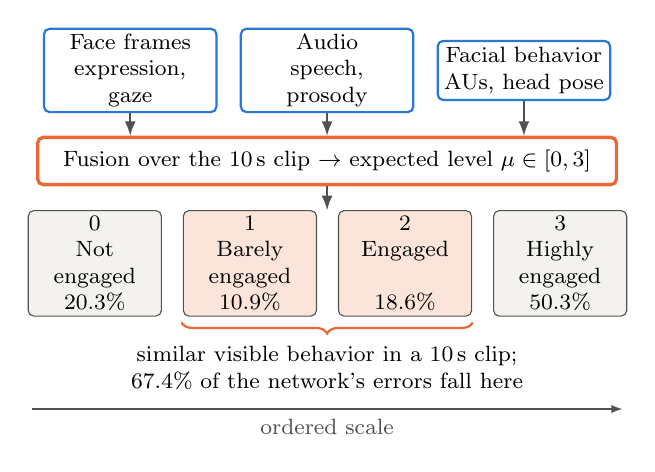
\begin{tikzpicture}[font=\footnotesize, >=latex,
  lvl/.style={draw=inkmuted, fill=boxfill, rounded corners=2pt, text width=1.55cm, minimum height=1.25cm, align=center, inner sep=2pt},
  cue/.style={draw=ours, thick, rounded corners=2pt, text width=2.05cm, minimum height=0.75cm, align=center, fill=white, inner sep=2pt}]
  \node[cue] (v) at (0.45,2.45) {Face frames\\expression, gaze};
  \node[cue] (a) at (2.95,2.45) {Audio\\speech, prosody};
  \node[cue] (b) at (5.45,2.45) {Facial behavior\\AUs, head pose};
  \node[draw=fused, very thick, rounded corners=2pt, minimum width=7.35cm, minimum height=0.6cm, fill=white, align=center] (m) at (2.95,1.3)
     {Fusion over the 10\,s clip $\rightarrow$ expected level $\mu\in[0,3]$};
  \foreach \s in {v,a,b} \draw[->, thick, inkmuted] (\s) -- (\s |- m.north);
  \node[lvl] (l0) at (0,0)    {0\\Not\\engaged\\20.3\%};
  \node[lvl, fill=fused!18] (l1) at (1.97,0) {1\\Barely\\engaged\\10.9\%};
  \node[lvl, fill=fused!18] (l2) at (3.94,0) {2\\Engaged\\\phantom{x}\\18.6\%};
  \node[lvl] (l3) at (5.91,0) {3\\Highly\\engaged\\50.3\%};
  \draw[->, thick, inkmuted] (m.south) -- (m.south |- l1.north);
  \draw[decorate, decoration={brace, amplitude=4pt, mirror}, fused, thick] (1.1,-0.75) -- (4.8,-0.75)
     node[midway, below=5pt, text=black, align=center]{similar visible behavior in a 10\,s clip;\\67.4\% of the network's errors fall here};
  \draw[->, inkmuted] (-0.8,-1.85) -- node[below, text=inkmuted]{ordered scale} (6.7,-1.85);
\end{tikzpicture}

\caption{Problem description. Face, audio and facial-behavior evidence from a 10\,s clip is fused into an expected level on the ordered four-level EngageNet scale. Percentages are the share of each level in the test split (2,256 clips); the two middle levels receive 67.4\% of the errors of our audio-visual network (three seeds pooled)}
\label{fig:concept}
\end{figure}

\ournet{} has three blocks (Fig.~\ref{fig:arch}). Block A is an audio-visual network in which an EfficientFace backbone \citep{zhao2021efficientface} encodes the face frames, a convolutional encoder encodes the log-mel spectrogram, and the two token sequences exchange information in three cross-modal attention stages. Block B contains two models that read the OpenFace descriptor of the same clip, summarized over 20 uniform segments: a gradient-boosting classifier and a small Transformer encoder. Block C averages the three probability vectors with fixed weights and decodes the expected level with thresholds fitted on the validation split. The main contributions of this paper are as follows:
\begin{enumerate}
\item The first audio-visual result on EngageNet, to our knowledge, with the audio tokens of each clip pooled onto its visual frame grid. Audio alone is no better than the majority-class predictor, yet removing it lowers top-1 accuracy in eight of nine trained networks.
\item An ordinal decoding rule, thresholds on the expected level fitted on validation, which adds 2.00 points over argmax decoding on the same weights.
\item A fixed-weight fusion of the network with two models on segment statistics of 22 OpenFace features, which reaches 70.29 $\pm$ 0.14\% test accuracy, whereas a behavior branch trained inside the network changes no metric.
\item A per-seed evaluation with four metrics, five ablation studies, the computational cost of every component and an analysis of the remaining errors.
\end{enumerate}
Section~\ref{sec:related} reviews related work, Section~\ref{sec:method} describes the method, Section~\ref{sec:exp} the experimental setup, Section~\ref{sec:results} the results, and Section~\ref{sec:conclusion} concludes.

\section{Related work}\label{sec:related}

\subsection{Student engagement recognition}\label{sec:rw_engagement}

Engagement recognition from video has been reviewed by \citet{qarbal2025review} and \citet{mandia2023review}, and \citet{theophilus2026review} compare shallow and deep learning approaches to learner engagement prediction by how their features are selected, extracted and engineered. DAiSEE \citep{gupta2016daisee} contains 9,068 clips of 112 users labeled for engagement, boredom, confusion and frustration. CMOSE \citep{wu2024cmose} contains 12,193 segments from online classes, of which 24.0\% contain speech; adding audio to its visual features raises accuracy by 0.41 points on the full test set and by 3.18 points on the subset with speech. Proposed engagement models include a multimodal facial-cues detection system for e-learning \citep{gupta2023facialcues}, multitask EfficientNet affective computing \citep{thiruthuvanathan2024multitask}, a class-attention video transformer \citep{ai2024classattention}, learning-attention characterization from head-pose sight estimation \citep{mo2024headpose}, a transformer that fuses several visual feature groups \citep{xie2025msctrans}, a hierarchical multimodal fusion framework \citep{qin2026glpfusion} and a multimodal framework for real-time detection and feedback in higher education \citep{zhao2026multimodal}. On DAiSEE, gradient boosting on OpenFace action units has been reported to outperform an end-to-end convolutional network \citep{das2025optimizing}. In our work, we use both a learned frame encoder and explicit OpenFace descriptors, and we add the audio track, which CMOSE shows to be useful where speech is present.

\subsection{Engagement recognition on EngageNet}\label{sec:rw_engagenet}

The EngageNet baselines \citep{singh2023engagenet} are an LSTM, a CNN-LSTM and a TCN on OpenFace gaze, head-pose and action-unit features (61.84, 65.16 and 65.60\% test accuracy), a Transformer on the same features (67.61\%), a Transformer on MARLIN features (65.2\%) and a Transformer that fuses both (66.5\%). The Transformer describes each of 20 uniform segments of a clip by the mean and standard deviation of its features. For the same baseline model, validation accuracy is 1.5--5.2 points higher than test accuracy. Later work reports validation accuracy only: 68.91\% for TCCT-Net on head-pose signals \citep{vedernikov2024tcct}, 71.24\% for an ordinal spatial-temporal graph network on facial landmarks \citep{abedi2024stgcn}, 73.58\% for the prior-guided PriorNet \citep{vedernikov2026priornet}, and 68.98\% for a variational encoder with multiple decoders that uses video only on EngageNet \citep{augusma2026vemd}. In our work, we report accuracy on the official test split, which makes our results comparable with the six baselines, and we add the audio track, which none of these studies uses.

\subsection{Audio-visual fusion and ordinal modeling}\label{sec:rw_av}

AVT-CA \citep{venkatraman2025avtca} fuses audio and video features with transformer cross-attention in both directions, attention bottlenecks restrict the exchange between modalities to a few shared tokens \citep{nagrani2021attention}, and face-and-speech emotion recognition has been built from convolutional and LSTM networks \citep{taware2025mer}. For the facial stream, lightweight expression encoders are common: EfficientFace \citep{zhao2021efficientface} combines a local-feature extractor with channel-spatial modulation, a truncated MobileNetV2 with patch extraction and channel attention reaches 93.64\% on RAF-DB with 0.79\,M parameters \citep{vu2026lightweightfer}, and fine-tuned EfficientNet features ranked by information gain have been classified with a nearest-neighbour rule \citep{tribedi2025featureselection}. The engagement levels are ordered: CMOSE trains with a ranking mechanism for this order \citep{wu2024cmose}, ordinal supervision has been used for engagement in collaborative learning \citep{tran2026ordinal}, and ordinal models over affect features \citep{abedi2024affect} and facial landmarks \citep{abedi2024stgcn} outperform their non-ordinal counterparts. In our work, we adopt the intermediate cross-attention fusion of AVT-CA with an EfficientFace encoder, pair it with classical classifiers on explicit descriptors as in two-stage pipelines \citep{tribedi2025featureselection}, train with an ordinal penalty, and measure how much an ordinal decoding rule alone changes accuracy on the same weights.

\section{Proposed method}\label{sec:method}

\subsection{Problem formulation}\label{sec:formulation}

The label set is $\{0, 1, \ldots, K-1\}$ with $K = 4$, where larger values mean higher engagement. For a clip with label $y$, a model produces class probabilities $p_k$. The usual decision rule is $\hat{y} = \arg\max_{k} p_k$, which ignores the position of each class on the scale. An ordered alternative first reduces the probabilities to the expected level using the following equation,
\begin{equation}
\mu = \sum_{k=0}^{K-1} k \, p_k \label{eq:mu}
\end{equation}
and cuts $\mu \in [0, K-1]$ with increasing thresholds $\tau_1 < \tau_2 < \tau_3$,
\begin{equation}
\hat{y} = \sum_{m=1}^{K-1} \mathbf{1}\!\left[\mu \geq \tau_m\right] \label{eq:thresh}
\end{equation}
Here, $\mathbf{1}[\cdot]$ is the indicator function, and the thresholds are fitted on the validation split, not learned during training. During training, the order is used by adding to the cross-entropy loss $\mathcal{L}_{\mathrm{CE}}$ a penalty that grows with the distance between the predicted and the true level,
\begin{equation}
\mathcal{L} = \mathcal{L}_{\mathrm{CE}} + \lambda \sum_{k} p_k \left| c_k - c_y \right|, \qquad c_k = \frac{k}{K-1} \label{eq:loss}
\end{equation}
where $c_k$ is the normalized position of level $k$ and $\lambda$ sets the weight of the distance term.

\subsection{Audio-visual cross-attention network}\label{sec:method_av}

The network (block A in Fig.~\ref{fig:arch}) follows the intermediate cross-attention fusion of AVT-CA \citep{venkatraman2025avtca}, in which each modality attends to the other at three stages, with $h = 8$ attention heads throughout. \emph{Audio encoder.} The audio of each clip is resampled to 22.05\,kHz and converted to a 64-bin log-mel spectrogram ($64 \times 431$ for a full clip). Two two-dimensional convolution blocks with 64 and 128 channels and $2 \times 2$ max pooling, followed by averaging over frequency, give the audio tokens $\mathbf{A}_1 \in \mathbb{R}^{128 \times 107}$. \emph{Visual encoder.} Each clip is sampled at 5 frames per second, which gives up to 50 face crops of $224 \times 224$ pixels detected with MTCNN. An EfficientFace backbone \citep{zhao2021efficientface}, initialized from weights trained for facial expression recognition on AffectNet-7, maps each frame to a 1024-dimensional embedding, and two one-dimensional convolutions give the visual tokens $\mathbf{V}_1 \in \mathbb{R}^{64 \times T_v}$, $T_v \le 50$.

\emph{Per-sample temporal alignment.} Without alignment, each visual token would attend over about two audio tokens describing the same instant. We therefore pool the valid audio steps of every sample onto the valid visual length of the same sample,
\begin{equation}
\tilde{\mathbf{A}}_1[:, j] = \frac{1}{|S_j|}\sum_{t \in S_j} \mathbf{A}_1[:, t], \qquad j = 1,\dots,T_v^{(i)}
\end{equation}
where $S_j$ is the $j$-th of $T_v^{(i)}$ equal-width windows over the valid audio steps of sample $i$. Padding is excluded before pooling and masked afterwards, so $\tilde{\mathbf{A}}_1 \in \mathbb{R}^{128 \times 50}$ for a full clip. We did not train a matched network without this step, so its effect is not measured here.

\emph{Cross-attention fusion.} With multi-head attention $\mathrm{MHA}(X_q, X_k)$, in which $X_q$ supplies the queries and $X_k$ the keys and values, the two directions of an exchange are
\begin{align}
\tilde{X}_a &= X_a + \mathrm{MHA}(X_a, X_v) \label{eq:xattn_a}\\
\tilde{X}_v &= X_v + \mathrm{MHA}(X_v, X_a) \label{eq:xattn_v}
\end{align}
The attention matrix in (\ref{eq:xattn_a}) has shape $T_a \times T_v$, so the two lengths need not match. The first exchange uses $X_a = \tilde{\mathbf{A}}_1$ and $X_v = \mathbf{V}_1$. A second convolutional stage then gives $\mathbf{A}_2 \in \mathbb{R}^{128 \times 12}$ and $\mathbf{V}_2 \in \mathbb{R}^{128 \times 50}$, a second exchange lets the 12 audio tokens and the 50 visual tokens attend to each other, and a final pair of cross-attention blocks forms the third exchange. Each stream is reduced over time by masked attention pooling to a 128-dimensional vector, and a linear layer maps their concatenation to the class probabilities $p_{\mathrm{AV}}$.

\emph{Modality dropout and objective.} During training, the whole token sequence of each modality is set to zero with probability 0.15 per sample, independently for audio and video, at the start of the first exchange; its effect is not measured here, but it makes the inference-time modality ablation of Section~\ref{sec:ablation} a condition seen in training. The network is trained with (\ref{eq:loss}), $\lambda = 0.15$ and label smoothing of 0.1.

\begin{figure*}[t]
\centering
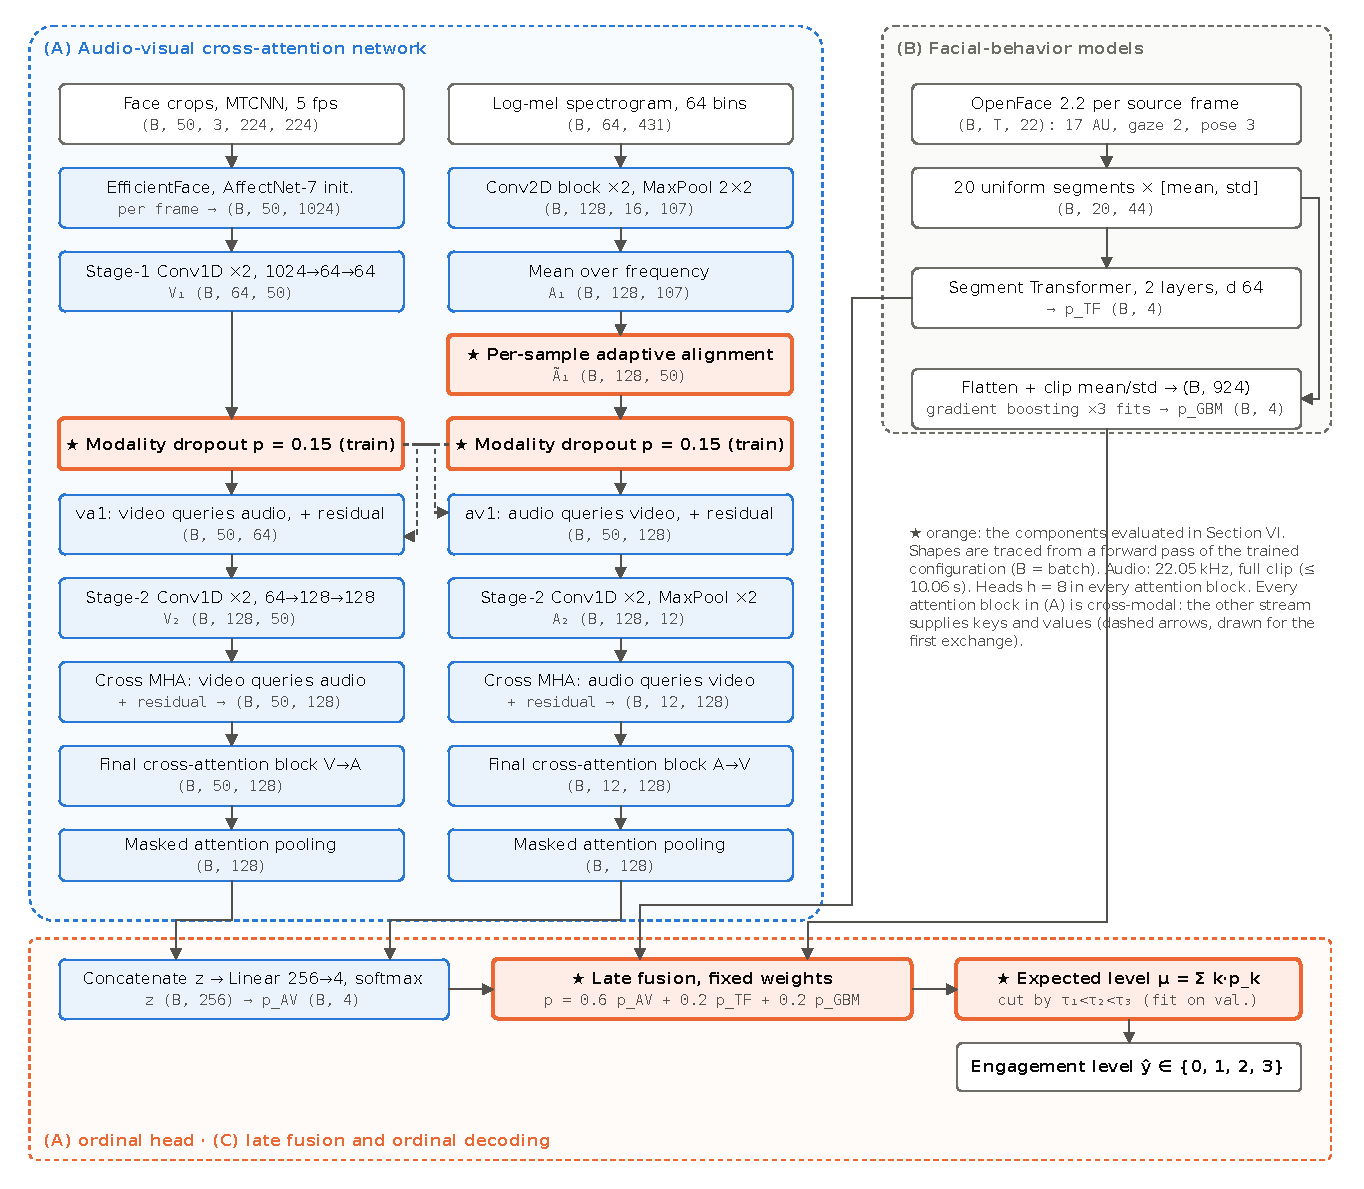
\includegraphics[width=\textwidth]{architecture}
\caption{Architecture of \ournet. Tensor shapes are traced from a forward pass of the trained configuration ($B$ = batch). (A) Audio tokens are pooled onto the 50-step visual clock of the same clip before the first cross-attention exchange; every attention block is cross-modal. (B) Two models on segment statistics of the per-frame OpenFace descriptor. (C) The three probability vectors are averaged with fixed weights, reduced to an expected level and cut by thresholds fitted on the validation split. Orange blocks mark the components evaluated in Section~\ref{sec:results}}
\label{fig:arch}
\end{figure*}

\subsection{Facial-behavior models}\label{sec:method_beh}

OpenFace 2.2 \citep{baltrusaitis2018openface} gives, per frame, 17 action-unit intensities, two gaze angles and three head-pose rotations, a 22-channel series. Following the best EngageNet baseline \citep{singh2023engagenet}, the series is divided into $S = 20$ segments of equal length, and each segment is described by the mean and standard deviation of every channel, a $20 \times 44$ token sequence. The \emph{gradient-boosting model} reads these tokens flattened together with the clip-level mean and standard deviation of each channel (924 dimensions); three histogram gradient-boosting fits with at most 15 leaves per tree, L2 regularization of 1.0, and learning rate and iteration count (0.05, 300), (0.03, 600) and (0.05, 300) are averaged to give $p_{\mathrm{GBM}}$. The \emph{segment Transformer} is a pre-norm encoder with a class token and learned positional embeddings (two layers, width 64, feed-forward width 128), trained with (\ref{eq:loss}) and random dropout of segment tokens; its size was selected from eight configurations by mean validation accuracy over three seeds, and it gives $p_{\mathrm{TF}}$.

\subsection{Late fusion and ordinal decoding}\label{sec:method_fusion}

Block C averages the three probability vectors,
\begin{equation}
p = w_{\mathrm{AV}}\, p_{\mathrm{AV}} + w_{\mathrm{TF}}\, p_{\mathrm{TF}} + w_{\mathrm{GBM}}\, p_{\mathrm{GBM}} \label{eq:late}
\end{equation}
with $(w_{\mathrm{AV}}, w_{\mathrm{TF}}, w_{\mathrm{GBM}}) = (0.6, 0.2, 0.2)$ for every seed, the setting that a grid search on the validation split selected for seven of the eight neural members we fused. We fuse probabilities because the three models are trained on different inputs with different learners, so their errors overlap less than those of networks fine-tuned from one checkpoint. The fused vector is decoded with (\ref{eq:mu}) and (\ref{eq:thresh}), with thresholds fitted by grid search on the validation split only. For the network alone we compare four decoders: argmax, argmax after a per-class logit bias fitted on validation, expected-level thresholds on a grid of step 0.05, and refined thresholds from a local search of radius 0.15 and step 0.005.

\section{Experimental setup}\label{sec:exp}

\subsection{Dataset}\label{sec:dataset}

In EngageNet \citep{singh2023engagenet}, participants aged 18 to 37 used a web platform with their own computer and webcam in computer labs, dorm rooms and open spaces; the videos were recorded at 640$\times$480 pixels or higher, and some contain background noise. We use the official subject-independent split of 90, 11 and 26 participants (7,983, 1,071 and 2,257 clips). Every source clip is at most 10.06\,s long, so the full clip is used for both modalities. We exclude the 105 clips labeled ``subject not present'' (104 training, 1 test). Table~\ref{tab:dataset} gives the clips per level; \emph{highly engaged} is 50.27\% of the test clips, so a majority-class predictor scores 50.27\% top-1 accuracy and 16.73 macro-F1.

\begin{table}[t]
\caption{EngageNet clips used, by engagement level (0 not engaged, 1 barely engaged, 2 engaged, 3 highly engaged)}\label{tab:dataset}
\begin{tabular*}{\columnwidth}{@{\extracolsep\fill}lccccc}
\toprule
Split & Clips & 0 & 1 & 2 & 3\\
\midrule
Training & 7,879 & 1,446 & 1,035 & 1,658 & 3,740\\
Validation & 1,071 & 132 & 97 & 273 & 569\\
Test & 2,256 & 457 & 246 & 419 & 1,134\\
Share (\%) & & 20.3 & 10.9 & 18.6 & 50.3\\
\botrule
\end{tabular*}
\end{table}

\subsection{Implementation details}\label{sec:impl}

Face frames were detected with MTCNN, cropped and resized to $224 \times 224$; clips shorter than 50 frames are padded with masked frames. OpenFace 2.2 detects a face in 98.8\% of the frames. The network was first trained on EngageNet in three stages from the AffectNet-7 initialization of the visual backbone (10 epochs at a learning rate of $10^{-2}$; a stage at $5 \times 10^{-4}$ with the ordinal objective and a class-balanced sampler; 8 epochs at $5 \times 10^{-5}$). All reported networks are fine-tuned from the resulting checkpoint for 6 epochs at $5 \times 10^{-5}$ with a step schedule, SGD with momentum 0.9 and weight decay $10^{-3}$, minibatch 8, the objective (\ref{eq:loss}) and a sampler that draws each clip with probability proportional to the inverse square root of its class frequency, with three random seeds; the checkpoint with the best validation top-1 accuracy is kept. Each run took about 32 minutes on one NVIDIA RTX 3090 GPU. The segment Transformer used AdamW (learning rate $10^{-3}$, weight decay 0.05, minibatch 64, dropout 0.3, 60 epochs). The behavior models were trained on the training split only. We used PyTorch 2.5 and scikit-learn. Only the decoding thresholds are fitted on validation, so each test result is computed once. Generative AI was used in preparing this study as described in the AI declaration in the Statements and Declarations; it did not produce data, and every number was computed by the authors' code from the trained models.

\subsection{Evaluation metrics}\label{sec:metrics}

For $N$ test clips with true levels $y_i$ and predictions $\hat{y}_i$, we report top-1 accuracy, $\frac{1}{N}\sum_i \mathbf{1}[\hat{y}_i = y_i]$, the metric of every EngageNet study; adjacent accuracy, $\frac{1}{N}\sum_i \mathbf{1}[|\hat{y}_i - y_i| \le 1]$; the mean absolute error in levels (MAE), $\frac{1}{N}\sum_i |\hat{y}_i - y_i|$; and macro-F1, the unweighted mean of the per-level F1 scores, which cannot be raised by predicting the majority level. Unless stated otherwise, a result is the mean over three seeds on the 2,256 test clips, the network alone is decoded with its refined thresholds, and $\pm$ values are standard deviations over seeds.

\section{Results and discussion}\label{sec:results}

\subsection{Comparison with published results}\label{sec:res_sota}

Fig.~\ref{fig:results} compares \ournet{} and its components with the six baselines released with EngageNet, the only published results on the official test split. \ournet{} reaches 70.29 $\pm$ 0.14\%, 2.68 points above the best baseline (67.61\%). The audio-visual network alone reaches 66.27 $\pm$ 0.45\%, above four of the six baselines and 1.34 points below the best one. The gradient-boosting model and the segment Transformer, which use a 22-dimensional subset of the 98-dimensional OpenFace features of the best baseline, reach 66.27\% and 66.99\%. The fusion gain comes from errors that the models do not share: the network is wrong on 33.3--34.2\% of the test clips (three seeds) and the gradient-boosting model on 33.7\%, but both are wrong on only 21.5--22.3\%.

\begin{figure}[t]
\centering
% Fig. -- test top-1 on EngageNet, one-column version with text >= 8 pt.
% Grey = published baselines (Singh et al., ICMI 2023, test split); blue = our single models; orange = fusions.
% Error bars: sd over three seeds. Values: results/fullclip (plan.md Sec. 19) and results/paper_springer/analysis.json.
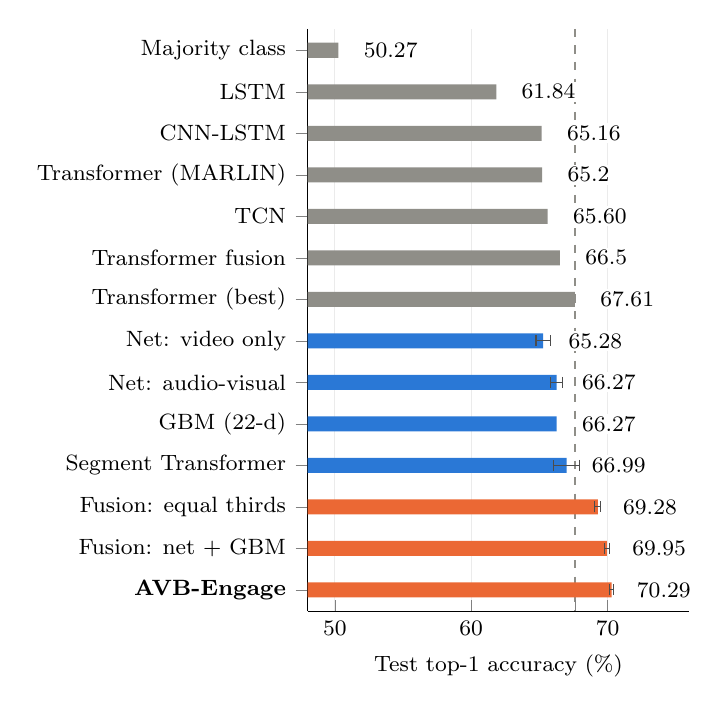
\begin{tikzpicture}
\begin{axis}[
  xbar, bar shift=0pt, scale only axis, width=0.40\columnwidth, height=7.4cm, bar width=5.5pt,
  xmin=48, xmax=76, xlabel={Test top-1 accuracy (\%)}, xlabel style={font=\footnotesize},
  xtick={50,60,70}, xticklabel style={font=\footnotesize}, yticklabel style={font=\footnotesize, align=right},
  ytick={maj,lstm,cnnlstm,marlin,tcn,tffus,tfbest,vonly,av,gbm,tf,eq3,av2,w3},
  symbolic y coords={maj,lstm,cnnlstm,marlin,tcn,tffus,tfbest,vonly,av,gbm,tf,eq3,av2,w3},
  yticklabels={Majority class,LSTM,CNN-LSTM,Transformer (MARLIN),TCN,Transformer fusion,Transformer (best),Net: video only,Net: audio-visual,GBM (22-d),Segment Transformer,Fusion: equal thirds,Fusion: net + GBM,\textbf{AVB-Engage}},
  y dir=reverse, enlarge y limits=0.04,
  axis x line*=bottom, axis y line*=left, xmajorgrids, grid style={draw=black!8},
  nodes near coords, nodes near coords style={font=\footnotesize, text=black, anchor=west, xshift=8pt, fill=white, inner sep=1pt},
  point meta=explicit symbolic,
  error bars/x dir=both, error bars/x explicit, error bars/error bar style={black!70},
  extra x ticks={67.61}, extra x tick labels={}, extra x tick style={grid=major, grid style={dashed, published, thick}},
]
\addplot[fill=published, draw=none] coordinates {
  (50.27,maj)[50.27] (61.84,lstm)[61.84] (65.16,cnnlstm)[65.16] (65.20,marlin)[65.2]
  (65.60,tcn)[65.60] (66.50,tffus)[66.5] (67.61,tfbest)[67.61]};
\addplot[fill=ours, draw=none] coordinates {
  (65.28,vonly) +- (0.53,0) [65.28] (66.27,av) +- (0.45,0) [66.27]
  (66.27,gbm)[66.27] (66.99,tf) +- (0.93,0) [66.99]};
\addplot[fill=fused, draw=none] coordinates {
  (69.28,eq3) +- (0.23,0) [69.28] (69.95,av2) +- (0.20,0) [69.95] (70.29,w3) +- (0.14,0) [70.29]};
\end{axis}
\end{tikzpicture}

\caption{Test top-1 accuracy on EngageNet. Grey: published test-split baselines \citep{singh2023engagenet}, all video-only, on OpenFace gaze, head-pose and action-unit features unless MARLIN is named. The dashed line marks the best baseline (67.61\%). Blue: our single models. Orange: our probability-level fusions. Error bars: standard deviation over three seeds}
\label{fig:results}
\end{figure}

Table~\ref{tab:seeds} reports every model per seed. \ournet{} has the highest top-1 accuracy and macro-F1, the lowest MAE (0.401) and the smallest spread over seeds (0.14). The network has the highest adjacent accuracy (91.55\%). For every model, adjacent accuracy is more than 20 points above top-1 accuracy, so most errors are one-level errors.

\begin{table*}[t]
\caption{Test results per seed (top-1, \%) and over three seeds. The rows with one input at inference are the ablation of Section~\ref{sec:abl_modality}; the gradient-boosting model is one averaged model}\label{tab:seeds}
\begin{tabular*}{\textwidth}{@{\extracolsep\fill}lccccccc}
\toprule
Model & Seed 1 & Seed 2 & Seed 3 & Top-1 & Adj. & MAE & Macro-F1\\
\midrule
Majority-class predictor & 50.27 & 50.27 & 50.27 & 50.27 & 68.84 & 1.012 & 16.73\\
Network, audio only & 46.59 & 50.27 & 50.27 & 49.04 $\pm$ 2.12 & 69.27 & 1.004 & 17.35\\
Network, video only & 65.60 & 65.56 & 64.67 & 65.28 $\pm$ 0.53 & 90.77 & 0.459 & 51.29\\
Audio-visual network & 65.78 & 66.36 & 66.67 & 66.27 $\pm$ 0.45 & \textbf{91.55} & 0.440 & 52.31\\
Gradient boosting & 66.27 & 66.27 & 66.27 & 66.27 & 89.01 & 0.476 & 50.04\\
Segment Transformer & 67.02 & 67.91 & 66.05 & 66.99 $\pm$ 0.93 & 87.90 & 0.487 & 49.45\\
\textbf{\ournet} & 70.17 & 70.26 & 70.43 & \textbf{70.29 $\pm$ 0.14} & 91.06 & \textbf{0.401} & \textbf{53.95}\\
\botrule
\end{tabular*}
\end{table*}

\subsection{Effect of the decoding rule}\label{sec:res_decoder}

Table~\ref{tab:decoder} isolates the decoding rule on the same trained weights. Expected-level thresholds add 2.00 points of top-1 accuracy over argmax for the network and 1.80 points for its video-only condition, with no test data used in the fit. This gain is larger than the effect of any training change we tested (Section~\ref{sec:abl_other}).

\begin{table}[t]
\caption{Decoding rule on the same weights (test top-1, \%)}\label{tab:decoder}
\begin{tabular*}{\columnwidth}{@{\extracolsep\fill}lcc}
\toprule
Decoder & Audio + video & Video only\\
\midrule
Argmax & 64.27 $\pm$ 0.22 & 63.48 $\pm$ 0.35\\
Logit bias & 65.06 $\pm$ 0.37 & 63.83 $\pm$ 0.45\\
Expected thr. & \textbf{66.34 $\pm$ 0.50} & 65.26 $\pm$ 0.40\\
Refined thr. & 66.27 $\pm$ 0.45 & \textbf{65.28 $\pm$ 0.53}\\
\botrule
\end{tabular*}
\end{table}

\subsection{Ablation studies}\label{sec:ablation}

Three seeds of one configuration give a standard deviation of 0.45 points of top-1 accuracy, and the binomial 95\% confidence interval on 2,256 clips is about $\pm$1.95 points. We therefore treat differences in three-seed means below about one point as within noise and rely on the consistency of sign across matched models for smaller effects.

\subsubsection{Contribution of each modality}\label{sec:abl_modality}

We kept the trained weights unchanged and set the tokens of one modality to zero at inference, the same operation as modality dropout, in the nine fine-tuned networks of this work (three seeds of the network and of the two behavior-branch variants of Section~\ref{sec:abl_branch}). Audio alone scores at or below the majority-class predictor in all nine networks (Table~\ref{tab:modality}), so audio carries no clip-level engagement signal on its own. Removing audio from the fused input lowers top-1 accuracy in eight of the nine networks, by 0.74 points on average. No single difference exceeds the noise floor, but the sign is consistent and reproduces an earlier sweep in which the audio-visual input scored higher than the video-only input in twelve of thirteen matched checkpoints.

\begin{table}[t]
\caption{Modality ablation at inference (nine networks, test top-1, \%)}\label{tab:modality}
\begin{tabular*}{\columnwidth}{@{\extracolsep\fill}lcc}
\toprule
Input at inference & Top-1 & AV higher in\\
\midrule
Audio + video & \textbf{66.16} & --\\
Video only & 65.41 & 8 of 9\\
Audio only & 48.60 & 9 of 9\\
\botrule
\end{tabular*}
\end{table}

\subsubsection{Behavior branch inside the network}\label{sec:abl_branch}

We attached a behavior branch to the same warm start: a one-dimensional convolution and a bidirectional GRU encode the OpenFace series on the 50-step visual clock, the audio-visual summary attends over these tokens, and the clip mean of the descriptor passes through a linear layer; the new classifier columns start at zero, so fine-tuning starts exactly from the audio-visual network. A second variant adds a text rendering of the same action-unit series. Neither variant changes any metric by more than a fraction of the seed standard deviation (Table~\ref{tab:branch}). The same descriptors raise accuracy through the separate models of block B: with a behavior-branch network as the neural member, the fused accuracy is 69.9--70.4\%. The descriptors are informative, and the recurrent branch does not extract what the segment statistics provide.

\begin{table}[t]
\caption{Behavior branch inside the network (test, mean of three seeds; top-1 standard deviations 0.45, 0.59 and 0.59)}\label{tab:branch}
\begin{tabular*}{\columnwidth}{@{\extracolsep\fill}lccc}
\toprule
Network & Top-1 & Adj. & Macro-F1\\
\midrule
Audio-visual & \textbf{66.27} & 91.55 & \textbf{52.31}\\
+ behavior branch & 66.08 & 91.62 & 52.16\\
+ branch + AU text & 66.12 & \textbf{91.67} & 52.26\\
\botrule
\end{tabular*}
\end{table}

\subsubsection{Fusion weights and number of segments}\label{sec:abl_fusion}

Fig.~\ref{fig:sensitivity} shows the test accuracy as a function of the network's weight. In the two-way fusion with the gradient-boosting model, every weight from 0.5 to 0.7 gives 69.5--70.2\%; the three-way fusion is best at 0.6 and drops to 67.5\% at 0.8. Equal weights, which involve no selection, give 69.28 $\pm$ 0.23\%, and weights selected on validation give 69.43--70.29\%. A two-way fusion with the segment Transformer alone gives 68.69 $\pm$ 2.08\% because the Transformer's validation accuracy does not follow its test accuracy closely; adding the gradient-boosting model reduces the spread to 0.14 points. With the full 98-dimensional OpenFace descriptor of the best baseline, the gradient-boosting model alone reaches 68.88\%, above the published Transformer on the same features, but the three-way fusion does not improve (69.15 $\pm$ 0.83\%). Re-running the gradient-boosting model with $S \in \{1, 5, 10, 20, 40\}$ segments changes its top-1 accuracy by less than one point (66.27--67.29\%; macro-F1 47.94 at $S = 1$ and 50.57 at $S = 40$), and the three-way fusion stays at 70.21--70.64\%, so the result does not depend on the choice of $S = 20$.

\begin{figure}[t]
\centering
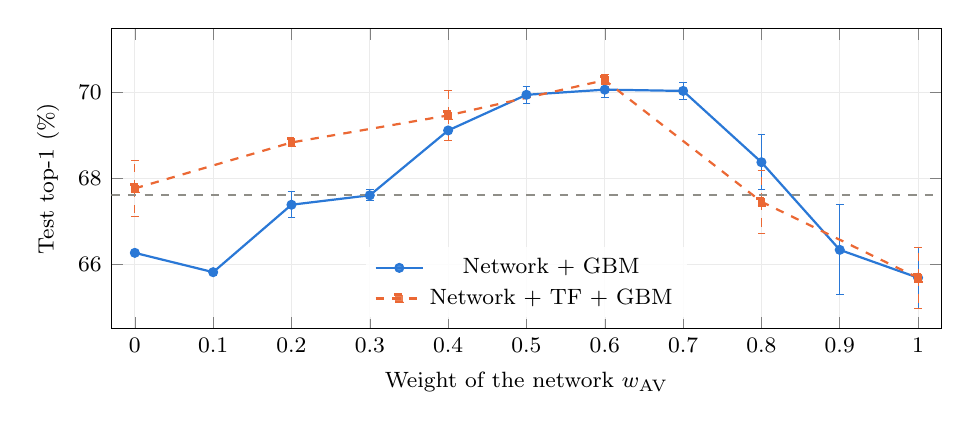
\begin{tikzpicture}
\begin{axis}[width=\columnwidth, height=5.4cm, xmin=-0.03, xmax=1.03, ymin=64.5, ymax=71.5,
  xlabel={Weight of the network $w_{\mathrm{AV}}$}, ylabel={Test top-1 (\%)},
  label style={font=\footnotesize}, tick label style={font=\footnotesize},
  legend style={font=\footnotesize, at={(0.5,0.03)}, anchor=south, draw=none, fill=white, fill opacity=0.85, text opacity=1},
  grid=major, grid style={draw=black!8}, error bars/y dir=both, error bars/y explicit]
\addplot[color=ours, mark=*, mark size=1.4pt, thick] coordinates {
 (0.0,66.27) +- (0,0) (0.1,65.82) +- (0,0.04) (0.2,67.39) +- (0,0.30) (0.3,67.61) +- (0,0.13) (0.4,69.12) +- (0,0.05)
 (0.5,69.95) +- (0,0.20) (0.6,70.07) +- (0,0.18) (0.7,70.04) +- (0,0.20) (0.8,68.38) +- (0,0.64) (0.9,66.34) +- (0,1.05) (1.0,65.69) +- (0,0.71)};
\addlegendentry{Network + GBM}
\addplot[color=fused, mark=square*, mark size=1.4pt, thick, dashed] coordinates {
 (0.0,67.77) +- (0,0.66) (0.2,68.84) +- (0,0.08) (0.4,69.47) +- (0,0.59) (0.6,70.29) +- (0,0.14) (0.8,67.46) +- (0,0.73) (1.0,65.69) +- (0,0.71)};
\addlegendentry{Network + TF + GBM}
\draw[dashed, published, thick] (axis cs:-0.03,67.61) -- (axis cs:1.03,67.61);
\end{axis}
\end{tikzpicture}
\caption{Fused test top-1 accuracy against the weight of the network (mean $\pm$ standard deviation over three seeds; thresholds fitted on validation for every weight). Two-way: $w_{\mathrm{GBM}} = 1 - w_{\mathrm{AV}}$. Three-way: $w_{\mathrm{TF}} = w_{\mathrm{GBM}} = (1 - w_{\mathrm{AV}})/2$. Dashed grey line: best published test result. At $w_{\mathrm{AV}} = 1$ the fusion threshold search gives 65.69\% instead of the network's 66.27\%}
\label{fig:sensitivity}
\end{figure}

\subsubsection{Training variables}\label{sec:abl_other}

Fourteen fine-tuning runs from the same checkpoint each changed one training variable: loss type, ordinal penalty weight, label smoothing, weight averaging, learning-rate schedule, SpecAugment, frame cap, synchronized random temporal cropping, class weighting and class-balanced sampling. Their standard deviation (0.52 points) is no larger than that of three seeds of one configuration (0.45 points); augmentation is the only variable with a clear direction, and it lowers accuracy (64.89\% against 65.82\% without cropping). Averaging the logits of all fourteen networks gives 65.69\%, below the best single network, because networks fine-tuned from one checkpoint make similar errors. The gains in this paper therefore come from the decoding rule and from combining different models, not from a training setting.

\subsection{Computational cost}\label{sec:res_cost}

Table~\ref{tab:cost} reports the size and inference cost per clip, measured on real test clips with batch size 1. The network has 2.38\,M parameters, 1.26\,M of them in the EfficientFace frame encoder, and needs 16.0\,GFLOPs per 10\,s clip, almost all in the frame encoder; the three cross-modal exchanges need about 0.04\,GFLOPs. The behavior models are small. The most expensive step is the OpenFace extraction that feeds block B, which needed a median of 11.3\,s per 300-frame clip on one CPU thread, about the length of the clip, so real-time use needs several threads or a faster extractor.

\begin{table}[t]
\caption{Size (parameters or trees) and inference time per 10\,s clip, batch size 1. GPU: RTX 3090; CPU: eight threads, except OpenFace on one thread. TF: segment Transformer; GBM: gradient boosting}\label{tab:cost}
\begin{tabular*}{\columnwidth}{@{\extracolsep\fill}lccc}
\toprule
Component & Size & GPU & CPU\\
\midrule
AV network & 2.38\,M & 21.5\,ms & 271\,ms\\
Segment TF & 71.6\,k & -- & 0.7\,ms\\
GBM & 4,800 trees & -- & 38.6\,ms\\
OpenFace & -- & -- & 11.3\,s\\
\botrule
\end{tabular*}
\end{table}

\subsection{Error analysis and limitations}\label{sec:res_errors}

Fig.~\ref{fig:confusion} shows the row-normalized confusion matrices pooled over three seeds. The network recognizes the extreme levels at 77\% and 87\% and the middle levels, \emph{barely engaged} and \emph{engaged}, at 18\% and 26\%. Of its errors, 74.9\% are off by one level and 67.4\% fall on the two middle levels, which make up 29.5\% of the test set. \ournet{} raises recall on \emph{highly engaged} from 87\% to 94\% and on \emph{engaged} from 26\% to 38\%, and lowers it on \emph{not engaged} (77\% to 73\%) and \emph{barely engaged} (18\% to 11\%). We see two reasons. First, the middle levels describe a difference of degree in similar visible behavior, and a ten-second clip of a student watching a recorded lecture contains no response to an instructor that would separate them; merging the two middle levels of the same network, without retraining, raises its argmax accuracy from 64.27\% to 70.70\% and its gain over the majority class from 13.97 to 20.40 points. Second, the label prior differs between splits (12.3\% \emph{not engaged} in validation, 20.3\% in test), so thresholds fitted on validation are not the best for test; thresholds fitted on the test split itself would give 67.82\% instead of 65.69\% for one network, an upper bound rather than a method.

\begin{figure}[t]
\centering
% Fig. -- row-normalised test confusion matrices (%), pooled over the three seeds (3 x 2,256 clips).
% Values: results/paper_springer/analysis.json (scripts/paper/springer_analysis.py). Network decoded with its
% refined expected-level thresholds; fusion with thresholds fitted on validation (fixed 0.6/0.2/0.2).
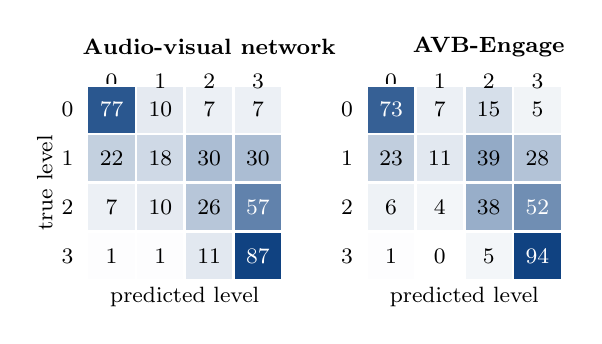
\begin{tikzpicture}[font=\footnotesize, cell/.style={minimum size=0.62cm, inner sep=0pt, draw=white, line width=1pt}]
\node[font=\footnotesize\bfseries] at (1.24,0.8) {Audio-visual network};
\node[anchor=east] at (-0.36,0.00) {0}; \node at (0.00,0.36) {0};
\node[cell, fill=seqhi!89!seqlo, text=white] at (0.00,0.00) {77};
\node[cell, fill=seqhi!11!seqlo] at (0.62,0.00) {10};
\node[cell, fill=seqhi!8!seqlo] at (1.24,0.00) {7};
\node[cell, fill=seqhi!8!seqlo] at (1.86,0.00) {7};
\node[anchor=east] at (-0.36,-0.62) {1}; \node at (0.62,0.36) {1};
\node[cell, fill=seqhi!25!seqlo] at (0.00,-0.62) {22};
\node[cell, fill=seqhi!20!seqlo] at (0.62,-0.62) {18};
\node[cell, fill=seqhi!35!seqlo] at (1.24,-0.62) {30};
\node[cell, fill=seqhi!35!seqlo] at (1.86,-0.62) {30};
\node[anchor=east] at (-0.36,-1.24) {2}; \node at (1.24,0.36) {2};
\node[cell, fill=seqhi!8!seqlo] at (0.00,-1.24) {7};
\node[cell, fill=seqhi!11!seqlo] at (0.62,-1.24) {10};
\node[cell, fill=seqhi!30!seqlo] at (1.24,-1.24) {26};
\node[cell, fill=seqhi!66!seqlo, text=white] at (1.86,-1.24) {57};
\node[anchor=east] at (-0.36,-1.86) {3}; \node at (1.86,0.36) {3};
\node[cell, fill=seqhi!1!seqlo] at (0.00,-1.86) {1};
\node[cell, fill=seqhi!1!seqlo] at (0.62,-1.86) {1};
\node[cell, fill=seqhi!12!seqlo] at (1.24,-1.86) {11};
\node[cell, fill=seqhi!100!seqlo, text=white] at (1.86,-1.86) {87};
\node at (0.93,-2.38) {predicted level};
\node[font=\footnotesize\bfseries] at (4.79,0.8) {AVB-Engage};
\node[anchor=east] at (3.19,0.00) {0}; \node at (3.55,0.36) {0};
\node[cell, fill=seqhi!84!seqlo, text=white] at (3.55,0.00) {73};
\node[cell, fill=seqhi!8!seqlo] at (4.17,0.00) {7};
\node[cell, fill=seqhi!17!seqlo] at (4.79,0.00) {15};
\node[cell, fill=seqhi!6!seqlo] at (5.41,0.00) {5};
\node[anchor=east] at (3.19,-0.62) {1}; \node at (4.17,0.36) {1};
\node[cell, fill=seqhi!26!seqlo] at (3.55,-0.62) {23};
\node[cell, fill=seqhi!12!seqlo] at (4.17,-0.62) {11};
\node[cell, fill=seqhi!45!seqlo] at (4.79,-0.62) {39};
\node[cell, fill=seqhi!32!seqlo] at (5.41,-0.62) {28};
\node[anchor=east] at (3.19,-1.24) {2}; \node at (4.79,0.36) {2};
\node[cell, fill=seqhi!7!seqlo] at (3.55,-1.24) {6};
\node[cell, fill=seqhi!5!seqlo] at (4.17,-1.24) {4};
\node[cell, fill=seqhi!43!seqlo] at (4.79,-1.24) {38};
\node[cell, fill=seqhi!60!seqlo, text=white] at (5.41,-1.24) {52};
\node[anchor=east] at (3.19,-1.86) {3}; \node at (5.41,0.36) {3};
\node[cell, fill=seqhi!1!seqlo] at (3.55,-1.86) {1};
\node[cell, fill=seqhi!0!seqlo] at (4.17,-1.86) {0};
\node[cell, fill=seqhi!5!seqlo] at (4.79,-1.86) {5};
\node[cell, fill=seqhi!100!seqlo, text=white] at (5.41,-1.86) {94};
\node at (4.48,-2.38) {predicted level};
\node[rotate=90] at (-0.85,-0.93) {true level};
\end{tikzpicture}

\caption{Row-normalized test confusion matrices (\%) of the audio-visual network (left) and \ournet{} (right), pooled over three seeds ($3 \times 2{,}256$ clips). Levels: 0 not engaged, 1 barely engaged, 2 engaged, 3 highly engaged}
\label{fig:confusion}
\end{figure}

This study has limitations. It uses one dataset, in which participants watch recorded lectures and rarely speak, so the audio contribution is small (0.74 points) and the speaking or listening role cannot be studied. The per-sample alignment and the modality dropout were not removed in a matched run. The fusion weights were selected on validation for seven of eight members, although equal weights still give 69.28\%. OpenFace extraction is slow on one thread, and we have not measured how well people separate the four levels on the same clips.

\section{Conclusion}\label{sec:conclusion}

We presented \ournet, which combines an audio-visual cross-attention network with two models on segment statistics of OpenFace descriptors and decodes the four ordered engagement levels through the expected level. On the official EngageNet test split it reached 70.29 $\pm$ 0.14\% top-1 accuracy, 91.06\% adjacent accuracy and an MAE of 0.401 levels, 2.68 points above the best published test result. Audio has no standalone signal on this dataset but raised accuracy in eight of nine networks when fused with video, threshold decoding added 2.00 points on the same weights, and the behavior descriptors helped through segment statistics in separate models rather than through a branch inside the network. Future work will evaluate the model on live online classes with per-participant audio, annotate the speaking or listening role of each student, and measure human agreement on the middle levels.

\backmatter

\section*{Statements and Declarations}

\bmhead{Funding}
% TODO (authors): replace if any funding was received.
The authors did not receive support from any organization for the submitted work.

\bmhead{Competing interests}
The authors have no relevant financial or non-financial interests to disclose.

\bmhead{Ethics approval and consent}
This study uses only the publicly released EngageNet dataset \citep{singh2023engagenet}; no new data were collected from human participants, and no images of participants are shown. % TODO (authors): add the EngageNet licence terms.

\bmhead{Data and code availability}
EngageNet is available from its authors under their access conditions. The per-clip predictions, derived features and code are available from the corresponding author on reasonable request. % TODO (authors): add a repository link if public.

\bmhead{Author contributions}
% TODO (authors): CRediT statement.
To be completed by the authors.

\bmhead{Use of generative AI}
% DRAFT -- the authors must review and edit this statement so that it is accurate.
The authors used Claude (Anthropic) under their direction to write and debug experiment and analysis code, to check bibliographic metadata, to generate the source code of the charts and of the architecture diagram from the authors' result files and model definition, and to draft and condense manuscript text from the authors' results and earlier drafts. All experiments were designed and run by the authors, every number was computed by the authors' code from the trained models, and the authors reviewed all text, figures and references and take full responsibility for the content.

\bibliography{references}

\end{document}
